\section{Annex}
\subsection{Source code}

\begin{listing}[H]
\inputminted[
    fontsize=\small,
    linenos]{erlang}{resources/src/server.erl}
\caption{server.erl}
\end{listing}

\begin{listing}[H]
\inputminted[
    fontsize=\small,
    linenos]{erlang}{resources/src/host.erl}
\caption{server.erl}
\end{listing}

\clearpage
\subsection{Screenshots}

%% Init
\begin{figure}[h!]
\centering
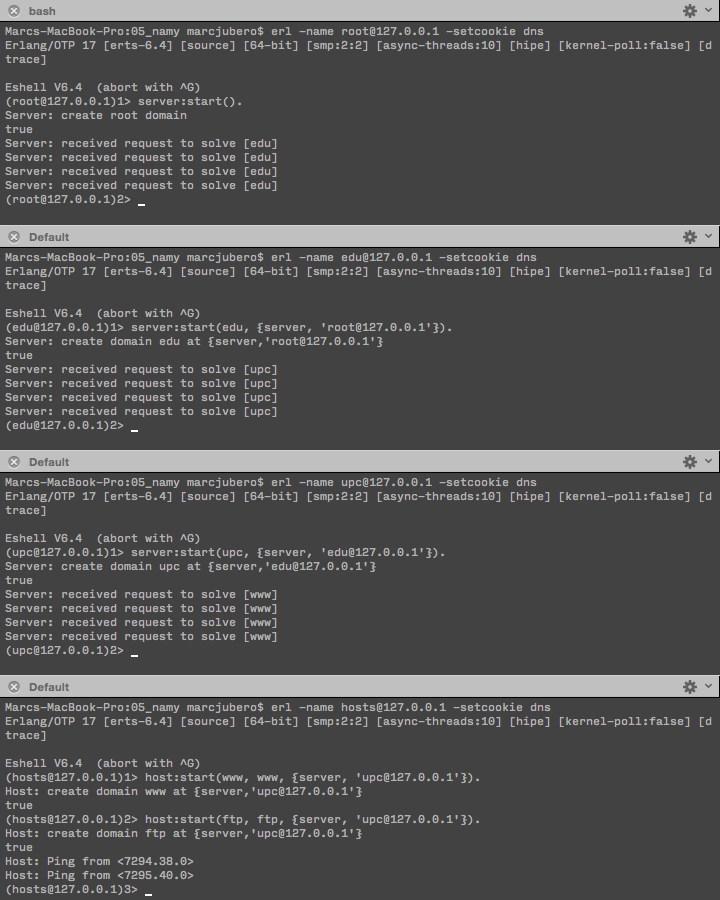
\includegraphics[scale=0.6]{resources/img/server+hosts_noCache.png}
\caption{Initial scenario}
\end{figure}

\begin{figure}[h!]
\centering
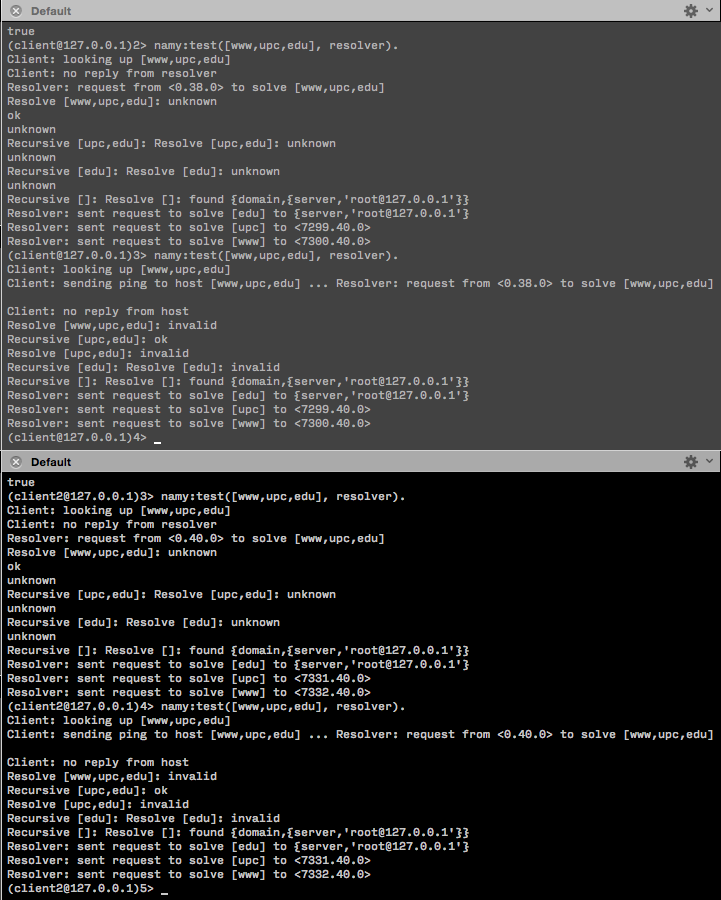
\includegraphics[scale=0.6]{resources/img/2clients_askingForName.png}
\caption{2 clients asking for a name}
\end{figure}

%% No cache experiments
\begin{figure}[h!]
\centering
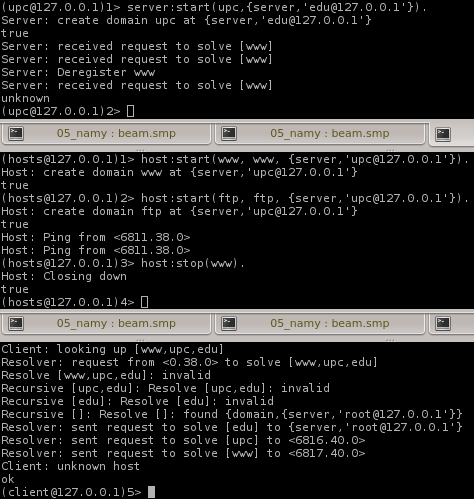
\includegraphics[scale=1]{resources/img/hostWWWdown_NoCache_deregisterParent.png}
\caption{Host WWW down, no cache \& deregister parent}
\end{figure}

\begin{figure}[h!]
\centering
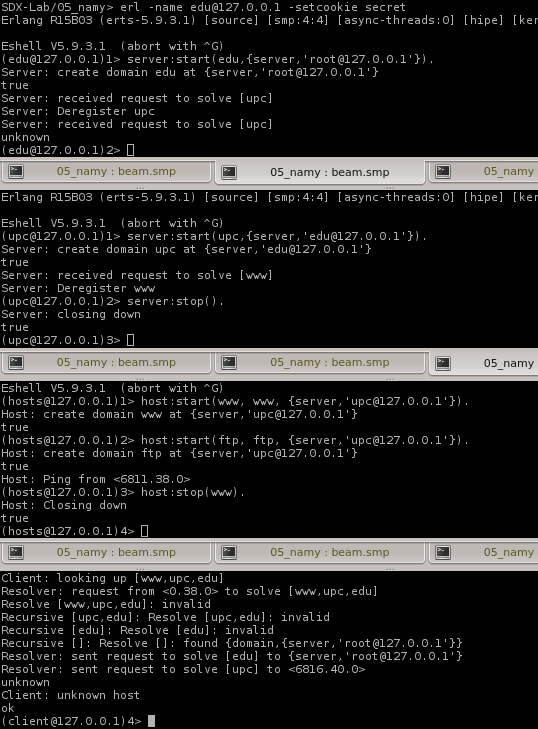
\includegraphics[scale=1]{resources/img/hostWWWdown_serverUPCdown_NoCache_deregisterParent.png}
\caption{Host WWW down, Server UPC down, no cache \& deregister parent}
\end{figure}

%% With cache

\begin{figure}[h!]
\centering
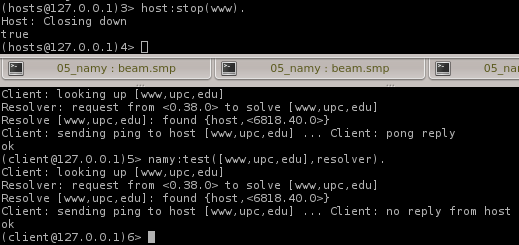
\includegraphics[scale=1]{resources/img/hostWWWdown_cache.png}
\caption{Host WWW down \& using cache}
\end{figure}

